\documentclass[twocolumn, a4paper, 10pt]{article}
\usepackage[cmex10]{amsmath}

% makes everything a bit tighter
\usepackage{microtype}

\usepackage{amsopn}
\usepackage{amsthm}
\usepackage{amsmath}

\usepackage{hyperref}

\usepackage{graphicx}
\graphicspath{{./figures/}}
\DeclareGraphicsExtensions{.pdf,.jpeg,.png,.eps, .svg}

% if you want to draw sth: have a look at tikz
\usepackage{tikz}
\usetikzlibrary{positioning}
\usetikzlibrary{calc, fit, shapes, decorations.markings, calendar}

% comments for yourself
\newcommand{\me}[1]{{\color{red}#1}}
% and on the margin
\newcommand{\meb}[1]{\marginpar{\small\textcolor{red}{#1}}}

% comments for benny
\newcommand{\cb}[1]{{\color{red}#1}}
% and on the margin
\newcommand{\cbb}[1]{\marginpar{\small\textcolor{red}{#1}}}

% for lorem ipsum - you can remove that
\usepackage{lipsum}

\begin{document}
\title{\Large Your Thesis Topic}

\author{
	Your Name
}

\maketitle

\def\abstractname{{\textbf Abstract}}
\begin{abstract}
{
\bfseries
This section should contain an abstract of your paper. The abstract's purpose is to report what your paper is about, and why the reader should bother to read the rest of it. It should be succinct and precise, but will usually also include a few sentences of motivation.
}
\end{abstract}


\section{Introduction}
\lipsum[1-3]
\section{About the Term Paper}
You may write your paper in english (preferred) or german. You \textbf{have} to use this template and \LaTeX, and should always submit the .pdf file, as well all the resources needed to build the .pdf file  (i.e.\ including all .tex/.bib-sources and images). Your final paper should be about 4-6 pages long (excluding bibliography). There will be two deadlines (see also the calendar in Figure~\ref{fig:calendar}):

\begin{figure}[t]
\centering
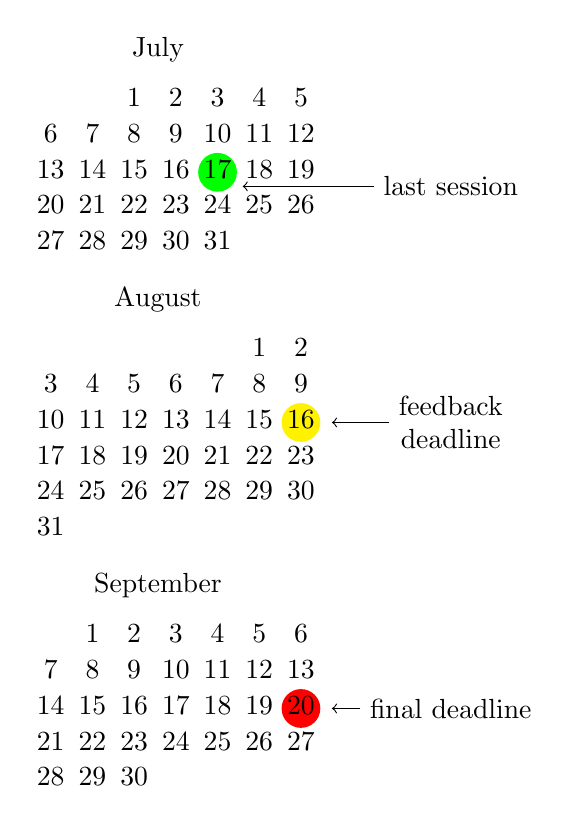
\begin{tikzpicture}
	\tikzstyle{every day}=[anchor=mid]
	\calendar[dates=2015-07-01 to 2015-09-30,week list, month label above centered]
	(calendar)
	if (equals=2015-07-17) {\node[fill=green, circle, minimum width=14pt] (start) {};}
	if (equals=2015-08-16) {\node[fill=yellow, circle, minimum width=14pt] (first) {};}
	if (equals=2015-09-20) {\node[fill=red, circle, minimum width=14pt] (final)  {};  
	};
	
	\node[right=0.5cm of final] (finalLabel) {final deadline};
	\draw[->, shorten >=4pt] (finalLabel) -- (final);
	\node[align=center] (firstLabel) at (first -| finalLabel) {feedback \\deadline};
	\draw[->, shorten >=4pt] (firstLabel) -- (first);
	\node (startLabel) at (start.south east -| firstLabel) {last session};
	\draw[->, shorten >=4pt] (startLabel) -- (start.south east);
\end{tikzpicture}
\caption{Calendar of deadlines for term papers. If requested, I will give feedback after the first deadline. The final deadline is \textbf{firm}: There will be no option to submit your paper after the final deadline.}
\label{fig:calendar}
\end{figure}

\begin{itemize}
\item feedback deadline: submit at least 1 filled page with title, abstract and introduction~\footnote{You are allowed to use ``lorem ipsum...'' to fill the page.} by
	\begin{center}
	\bfseries
		16.08.2015 23:59 CEST.
	\end{center}
\item final deadline: submit your final document by
	\begin{center}
	\bfseries
		20.09.2015 23:59 AoE.
	\end{center}
\end{itemize}

Both deadlines are mandatory (though you can always make your submission before the deadlines). 
\textbf{If} you request it, I will give you feedback on the document you submitted by the first deadline. I strongly recommend to use this opportunity.

If you run into any trouble writing your paper for whatever reason: please contact me as soon as possible. You can also ask me any questions by email, anytime.

\subsection{Topics and Themes}
You should already have a topic (or at least we discussed a few options and you are still deciding), if not please contact me as soon as possible. Topics \textbf{must} be be approved by me by email.  

There are four basic themes your topic fits in: Research proposal, survey article, introduction and investigation. I will describe those themes in more detail in the following sections.
If you have a favourite topic that does not fit in one of those themes: talk to me, we'll probably find a way to make it work. 

I recommend you to start with the most difficult or risky ones (research proposal and investigation). After an initial research phase (doing related work), you can fall back to the other alternatives if you don't get an idea you want to write about.  See Figure~\ref{fig:fallbackoptions} for an overview of the standard fallback options, but I will go into more detail in what follows.
 


\subsubsection{Research Proposal}
I strongly suggest everyone to try a research proposal first. If you try some time but didn't get a good idea: no problem. While thinking, you already did some research: just use that and go for the survey. 

You can think of a research proposal as some kind of advertisement for your own idea or research project. The proposal's goal is to convince the reader that your idea should be followed (and not the boring one from your colleagues / rivals).
It should contain
\begin{itemize}
	\item Motivation: What is the problem? Why is it important?
	\item Related work: which (scientific) papers discuss the same or similar ideas? How does the idea fit in the scientific literature?
	\item Novelty: What is new about the idea? How does it differ from the ideas published before?
	\item Idea: your idea in a succinct presentation, and finally a
	\item Research plan: How would you perform the actual research? How would you evaluate your idea / compare it to the related work?
\end{itemize}

\noindent What you need to do, is
\begin{enumerate}
	\item find a good idea (Caution: may be difficult),
	\item find out if the idea is new or someone else already had it (if so, refine your idea or go back to Step 1.) 
	\item write your idea down and work off the bullet points above.
\end{enumerate}
Note that your idea itself is not graded, since it is almost impossible to tell if an idea is ``good'' or ``bad''. The grade depends on the way the idea is processed according to the points above. In this sense:

\begin{center}
\bfseries
		Unorthodox / Crazy ideas welcome
\end{center}
\paragraph{Example topics}
\begin{itemize}
	\item Snails and Onions: Mixing Snail Mail for Fun and Profit\^{}WPrivacy
	\item Oblivious Blacklisting: OT meets Anonymous Credentials 
\end{itemize}

\subsubsection{Survey Article}
A survey article covers a broader topic, summarizes multiple papers and illustrates common elements and differences. The purpose of a survey article is to give the reader an overview of a particular topic (you read survey articles for a quick overview, either because you don't want to read every paper yourself just to know what’s going on, or you just want to find out which particular paper might be most relevant to your current problem). 

If you find out that there is an overwhelming amount of literature and that you won't be able to read all of it: no problem, you can switch to writing an introduction.

\textbf{ATTENTION}: If there is already a survey out there that covers your topic, your work should substantially add something. If in doubt: please notify me as soon as possible, we can always alter the topic slightly or you can go for the introduction.

\paragraph{Example topics}
\begin{itemize}
	\item A Survey of Data Anonymization Techniques
	\item State of the Art in Generic Multiparty Computation Protocols
\end{itemize}

\subsubsection{Introduction}
An introduction is very similar to a survey article, but only covers the most basic or important aspects of a topic. It's style and depth can be anything between the CACM articles we read in the seminar and MacKay's paper~\cite{mackay2005fountain} about fountain codes. It should give the reader (who is totally unfamiliar with the topic) a first glimpse and understanding of the topic: why it is interesting/important, how the most basic/important solutions work and what the open problems are. 

\paragraph{Example topics}
\begin{itemize}
	\item An Introduction to Location Privacy
	\item Password-based authenticated Key-Exchange - a Primer
\end{itemize}

\subsubsection{Investigation}
An investigation covers some project (some software), that is \textbf{not} already covered (published) in the scientific literature. Assume for example the project provides some privacy-guarantee. You
\begin{itemize}
	\item find out how it tries to achieve this goal,
	\item search for this approach in the scientific literature,
	\item compare the approach to solutions from the literature (are there better solutions?),
	\item evaluate the approach, and finally
	\item find out if and what could be done better.
\end{itemize}

\subsubsection*{Example papers}
For the research proposal and the survey, see my examples in KVV/Sakai. As a high quality example for an introduction, see the exemplary paper~\cite{mackay2005fountain} by MacKay about Fountain Codes. Sorry, I don't have a good example for an investigation right now.

\begin{figure}
\centering
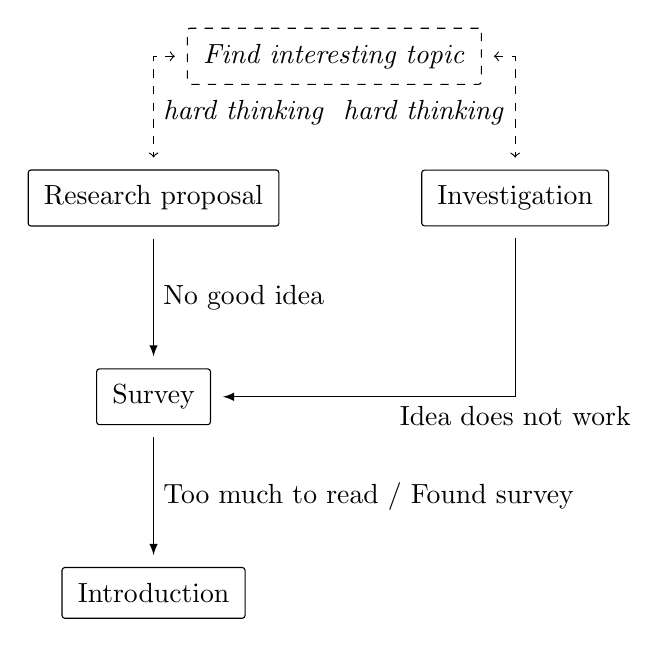
\begin{tikzpicture}
[
	node distance = 1.8cm,
	theme/.style={draw, rectangle, inner sep=0.2cm, rounded corners=1pt},
  	fallback/.style={->, -latex, shorten >=1ex, shorten <=1ex},
	fallbackT/.style={midway}
  ]
	\node[theme] (RP) {Research proposal};
	\node[theme, right=of RP] (Inv) {Investigation};
	
	\node[theme, dashed, above of=RP] (Start) at ($(RP) ! 0.5 ! (Inv)$) {\emph{Find interesting topic}};

	\node[theme, below=of RP] (Survey) {Survey};
	\node[theme, below=of Survey] (Intro) {Introduction};
	
	\draw[fallback] (Survey) -- (Intro) node[fallbackT, right] {Too much to read / Found survey};
	\draw[fallback] (RP) -- (Survey) node[fallbackT, right] {No good idea};
	\draw[fallback] (Inv) |- (Survey) node[fallbackT, below] {Idea does not work};

	\draw[fallback, dashed, <->] (Start) -| (RP) node[fallbackT, near end, right] (HT1) {\emph{hard thinking}};
	\draw[fallback, dashed, <->] (Start) -| (Inv) node[fallbackT, near end, left] (HT2) {\emph{hard thinking}};		
\end{tikzpicture}
\caption{Fallback opportunities for seminar theses.}
\label{fig:fallbackoptions}
\end{figure}


\subsubsection{Grading}
For every theme, the focus is on discovering, understanding and discussing scientific literature (related work). As a rule of thumb, ``related work'' and ``presentation quality'' are equally important (depending on your topic and theme, one or the other might be slightly more important)~\footnote{Details: of course, I am grading on a transient loop.}.

\section{Tips and Suggestions}
For writing in general, I suggest reading
\begin{itemize}
	\item \url{http://www.cs.indiana.edu/mit.research.how.to/section3.7.html}
\end{itemize}
Here
\begin{itemize}
	\item \url{http://www.cs.cmu.edu/afs/cs.cmu.edu/user/mleone/web/how-to.html}
\end{itemize}
is a nice collection of links on writing and research.
Regarding writing style, I found this page
\begin{itemize}
	\item \url{http://writingcenter.unc.edu/handouts/}
\end{itemize}
to be very helpful in general, and in particular these pages
\begin{itemize}
	\item \url{http://writingcenter.unc.edu/handouts/style/}, 
	\item \url{http://writingcenter.unc.edu/handouts/passive-voice/}.
\end{itemize}


\subsection{Writing Style}
These are some general tips regarding writing style. Regarding language and content, it is considered good style to
\begin{itemize}
	\item prefer active over of passive voice, 
	\item prefer short and easy sentences, 
	\item have consistent heading-styles (capitalization),
	\item keep discussion and reporting separated,
	\item reference every figure and table in your text, so that \LaTeX{} can find the right position for every graphic, and
	\item consider bullet points (as well as equations) to be part of a sentence.
\end{itemize}
There are a few common typesetting pitfalls many people make (alas, you even see them in research papers). You can avoid them, if you 
\begin{itemize}
	\item use \texttt{\textbackslash{}operatorname} and \texttt{\textbackslash{}text} for multi-character symbols in math mode (if needed):
		\begin{align*}
			\texttt{\textbackslash{}operatorname} \text{ is } \operatorname{GoodForOperators} \\
			 \texttt{\textbackslash{}text} \text{ is } \text{Good for text} \\
			 \text{the mistake } often\ produces\ bad\ spacing
		\end{align*}
		(Notice the spacing in ``often'', ``produces''),
	\item glue every reference/citation to the word in front using the tilde $\mathtt{\sim}$ symbol, so that numbers don't end up lonely at the beginning of a line,
	\item and if you abbreviate something: make sure to add a normal space after the ``.'' symbol:
		\begin{itemize}
			\item[] good abbrv.\ spacing
			\item[] bad abbrv. spacing
		\end{itemize}
		(Notice the larger space in the second case.)
\end{itemize}
\subsection{Graphics}
If you want to include a drawing in your document: have a look at the tikz library. It may be painful in the beginning, but  it's worth a try. See figures~\ref{fig:calendar} or~\ref{fig:fallbackoptions} for examples in this document or the texample web page\footnote{\url{http://www.texample.net/tikz/} Accessed: 2015-17-07}. 

Apart from being free and vector-graphics, it's based on \LaTeX{} and pgf. This way you can use all \LaTeX{} features (and your custom commands) in your graphics, as well as get automatically the same fonts, math-fonts, etc.\ as in the rest of your paper. 


\subsection{Data}

\begin{figure}
	\input{figures/days}
	\caption{Total number of request for the root page on the wiki per weekday. As expected, the number of requests grows exponentially as the week approaches the seminar dates on Friday.}
	\label{plot:weekdays}
\end{figure}

For the same reasons I really like tikz for graphics (consistent style, fonts, etc.), I also like gnuplot to plot data.
See figure~\ref{fig:weekdays} or the figures below as examples. 

If you configure gnuplot to output .tex and .eps files, you can just include the .tex file and get the same consistent look in your plots as in the rest of your document.


\section{Seminar wrap-up}
For your convenience, here is the list of papers we read in the privacy seminar: we did read~\cite{
solove2011privacy,
brin1999transparent,
oulasvirta2012long,
chaum1985security,
narayanan2013happened1,
narayanan2013happened2,
chaum1981untraceable,
dingeldine2004tor,
wolinsky2013hang,
juarez2014critical,
Mor2015bloom4,
yekhanin2010private,
camenisch2012electronic,
gervais2014privacy,
bonneau2014mixcoin,
starov2015measuring,
sweeney2002k,
nissenbaum2011contextual,
nissenbaum2004privacy,
narayanan2011link,
dwork2011differential,
homer2008resolving,
kelley2009nutrition,
reznichenko2014private,
kaptein2012rethinking,
afroz2014doppelganger,
chaum2004secret,
acquisti2015privacy,
jagatic2007social,
kang2011self}.

In the cryptography seminar, we did read or talk about~\cite{
koblitz2007another,
koblitz2007another2,
chatterjee2012another,
blum1983coin,
goldwasser1985knowledge,
rabin2005exchange,
rogaway2009practice,
koblitz2007uneasy,
bellare1998practice,
goldreich1987play,
fischer1996secure,
even1985randomized,
shamir1979share,
lindell2009proof,
holzer2012secure,
yao1986generate,
ben2008fairplaymp,
chaum1988multiparty,
rivest2001leak,
kushilevitz1997replication,
yekhanin2010private,
benaloh1994one,
miers2013zerocoin,
stefanov2013path,
bernstein2009introduction,
shor1997polynomial,
fiat1994broadcast,
micciancio2011lattice,
chor1994tracing,
juels2014honey,
blocki2014human,
di2005secure}.

\subsection*{Wiki access Logs (privacy seminar)}
I only had a brief look at the wiki logs, yet. Anyway, there are a few things that are worth sharing. 

\paragraph{Sanitization and Filtering} 
Before extracting data, I excluded any access to the wiki that didn't came through tor. I myself usually (with only very few exceptions) accessed the wiki through LAN/VPN, so this effectively filters out all but a few of my own requests. 

In the remaining entries I counted all user-agent strings found. Figure~\ref{fig:user_agents} and Table~\ref{table:user_agents} are based on this result.

After observing that some students may be trackable, I sanitized the remaining entries by removing all user-agent strings (see the \texttt{wiki\_sanitized.access} file in the \texttt{data/} folder) and every request that wasn't authenticated as ``anonymous''.

To mitigate over-counting, I then removed every request that wasn't to the wiki's home page (\texttt{?node=home}). There however still remains some overcounting (editing a node makes at least two requests to that node). The remaining figures (Figure~\ref{fig:days},~\ref{plot:weekdays} and~\ref{fig:weeks}) are based on those requests.

\paragraph{Results and Discussion}
Firstly, most of you seem to use a recent Tor Browser Bundle. Figure~\ref{fig:user_agents} shows that the majority of students include the same user-agent in web requests on the wiki. You can find the full list of user agents in Table~\ref{table:user_agents}. 

Secondly, it seems that some of you did not use the Tor Browser Bundle, but instead configured tor yourself in order to use with your favourite web browser. The data suggests that those browsers (e.g.\ ID 7) are trackable. 


\begin{figure}
	\input{figures/user_agents}
	\caption{Number of requests for each user-agent found in the wiki's access log. The vast majority of students seem to use a current Tor Browser Bundle, which identifies as Windows 7 (NT 6.1) (See Table~\ref{table:user_agents} for all user-agent strings and their IDs).}
	\label{fig:user_agents}
\end{figure}

\begin{table*}
\centering
\small
\begin{tabular}{lllp{0.7\linewidth}}
	ID & Count & Percent & User Agent\\
	\hline
	\input{figures/user_agents_table}
\end{tabular}
\caption{Detailed listing of all user-agent strings found (every request counted). All Browsers identify as Mozilla 5.0. The vast majority of students use the same web browser (a recent Tor Browser Bundle). There are however a few older versions and a few exotic exceptions. Noteworthy are IDs 7 and 2,3,4, which leak the browsers' language preference.}
\label{table:user_agents}
\end{table*}


\begin{figure*}
	\hfill
		\begin{minipage}{0.49\textwidth}
			\input{figures/weeks}
		\end{minipage}
	\hfill
		\begin{minipage}{0.49\textwidth}
			\input{figures/weeks_zoom}
		\end{minipage}
	\hfill
	
	\caption{Access on the wiki for each week by week day, divided by 12h ticks and starting at Monday 00:00. About half of the requests happened on Friday, starting a bit before noon, and continuing through the afternoon, however stopping before 18:00.}
	\label{fig:weeks}
\end{figure*}

\begin{figure}
	\input{figures/days_sorted}
	\caption{Shows cumulative distribution of access requests to the wiki's home page by time of day.}
	\label{fig:days}
\end{figure}


Apart from user-agents I also took a brief look at access times. Figure~\ref{plot:weekdays} indicates that the majority of requests have been made on Friday. In a more closer look, the cumulative distribution of requests in Figure~\ref{fig:weeks} reveals that the highest peek of requests happened right before or during the seminar sessions. These requests also dominate if we aggregates all days together and only look at the time of day a request occured, as Figure~\ref{fig:days} indicates.


{
	\bibliographystyle{plain}
	\bibliography{bibliography,privacy,crypto}
}

\appendix
\end{document}


